%% Use the hmcposter class with the thesis document-class option.
\documentclass[thesis]{hmcposter}
\usepackage{graphicx}
\usepackage{natbib}
\usepackage{booktabs}
\usepackage{subfig}
\usepackage{amsmath}
\usepackage{textcomp}
\usepackage{url}

%% Author of the thesis.
\author{Claire Connelly}

%% The year of your thesis poster's creation.
\posteryear{2015}

%% Thesis Title.
\title{Putting Together a Poster\\for Presentation Days}

%% The name of the class for which the poster was created.
%% Generally we see posters for thesis and Clinic, but sometimes
%% other classes require or allow the creation of posters to
%% communicate the results of a project.
%% 
%% Use the format Math nnn: Class Title.
\class{Math 197: Senior Thesis}

%% Advisor(s) name or names.  Separate with \and.
\advisor{Melissa O'Neill \and Lesley Ward}

%% Reader(s) name or names.  Separate with \and.
\reader{Melissa O'Neill \and Charlie Watts}


%% Define the \BibTeX command, used in our example document.
\providecommand{\bibtex}{{\rmfamily B\kern-.05em%
    \textsc{i\kern-.025em b}\kern-.08em%
    T\kern-.1667em\lower.7ex\hbox{E}\kern-.125emX}}


\pagestyle{fancy}

\begin{document}

\begin{poster}

\section{Introduction}
% Note that we're not labeling sections because you shouldn't be
% doing a lot of referring back and forth in your poster---let the
% interested folks read your thesis or Clinic report, or ask
% questions.

Describe the basics about your thesis or project here---briefly!  An
image such as Figure~\ref{fig:our-poster} can help jazz up the
introduction and get people interested in your poster.

\begin{figure}
\begin{center}
\fbox{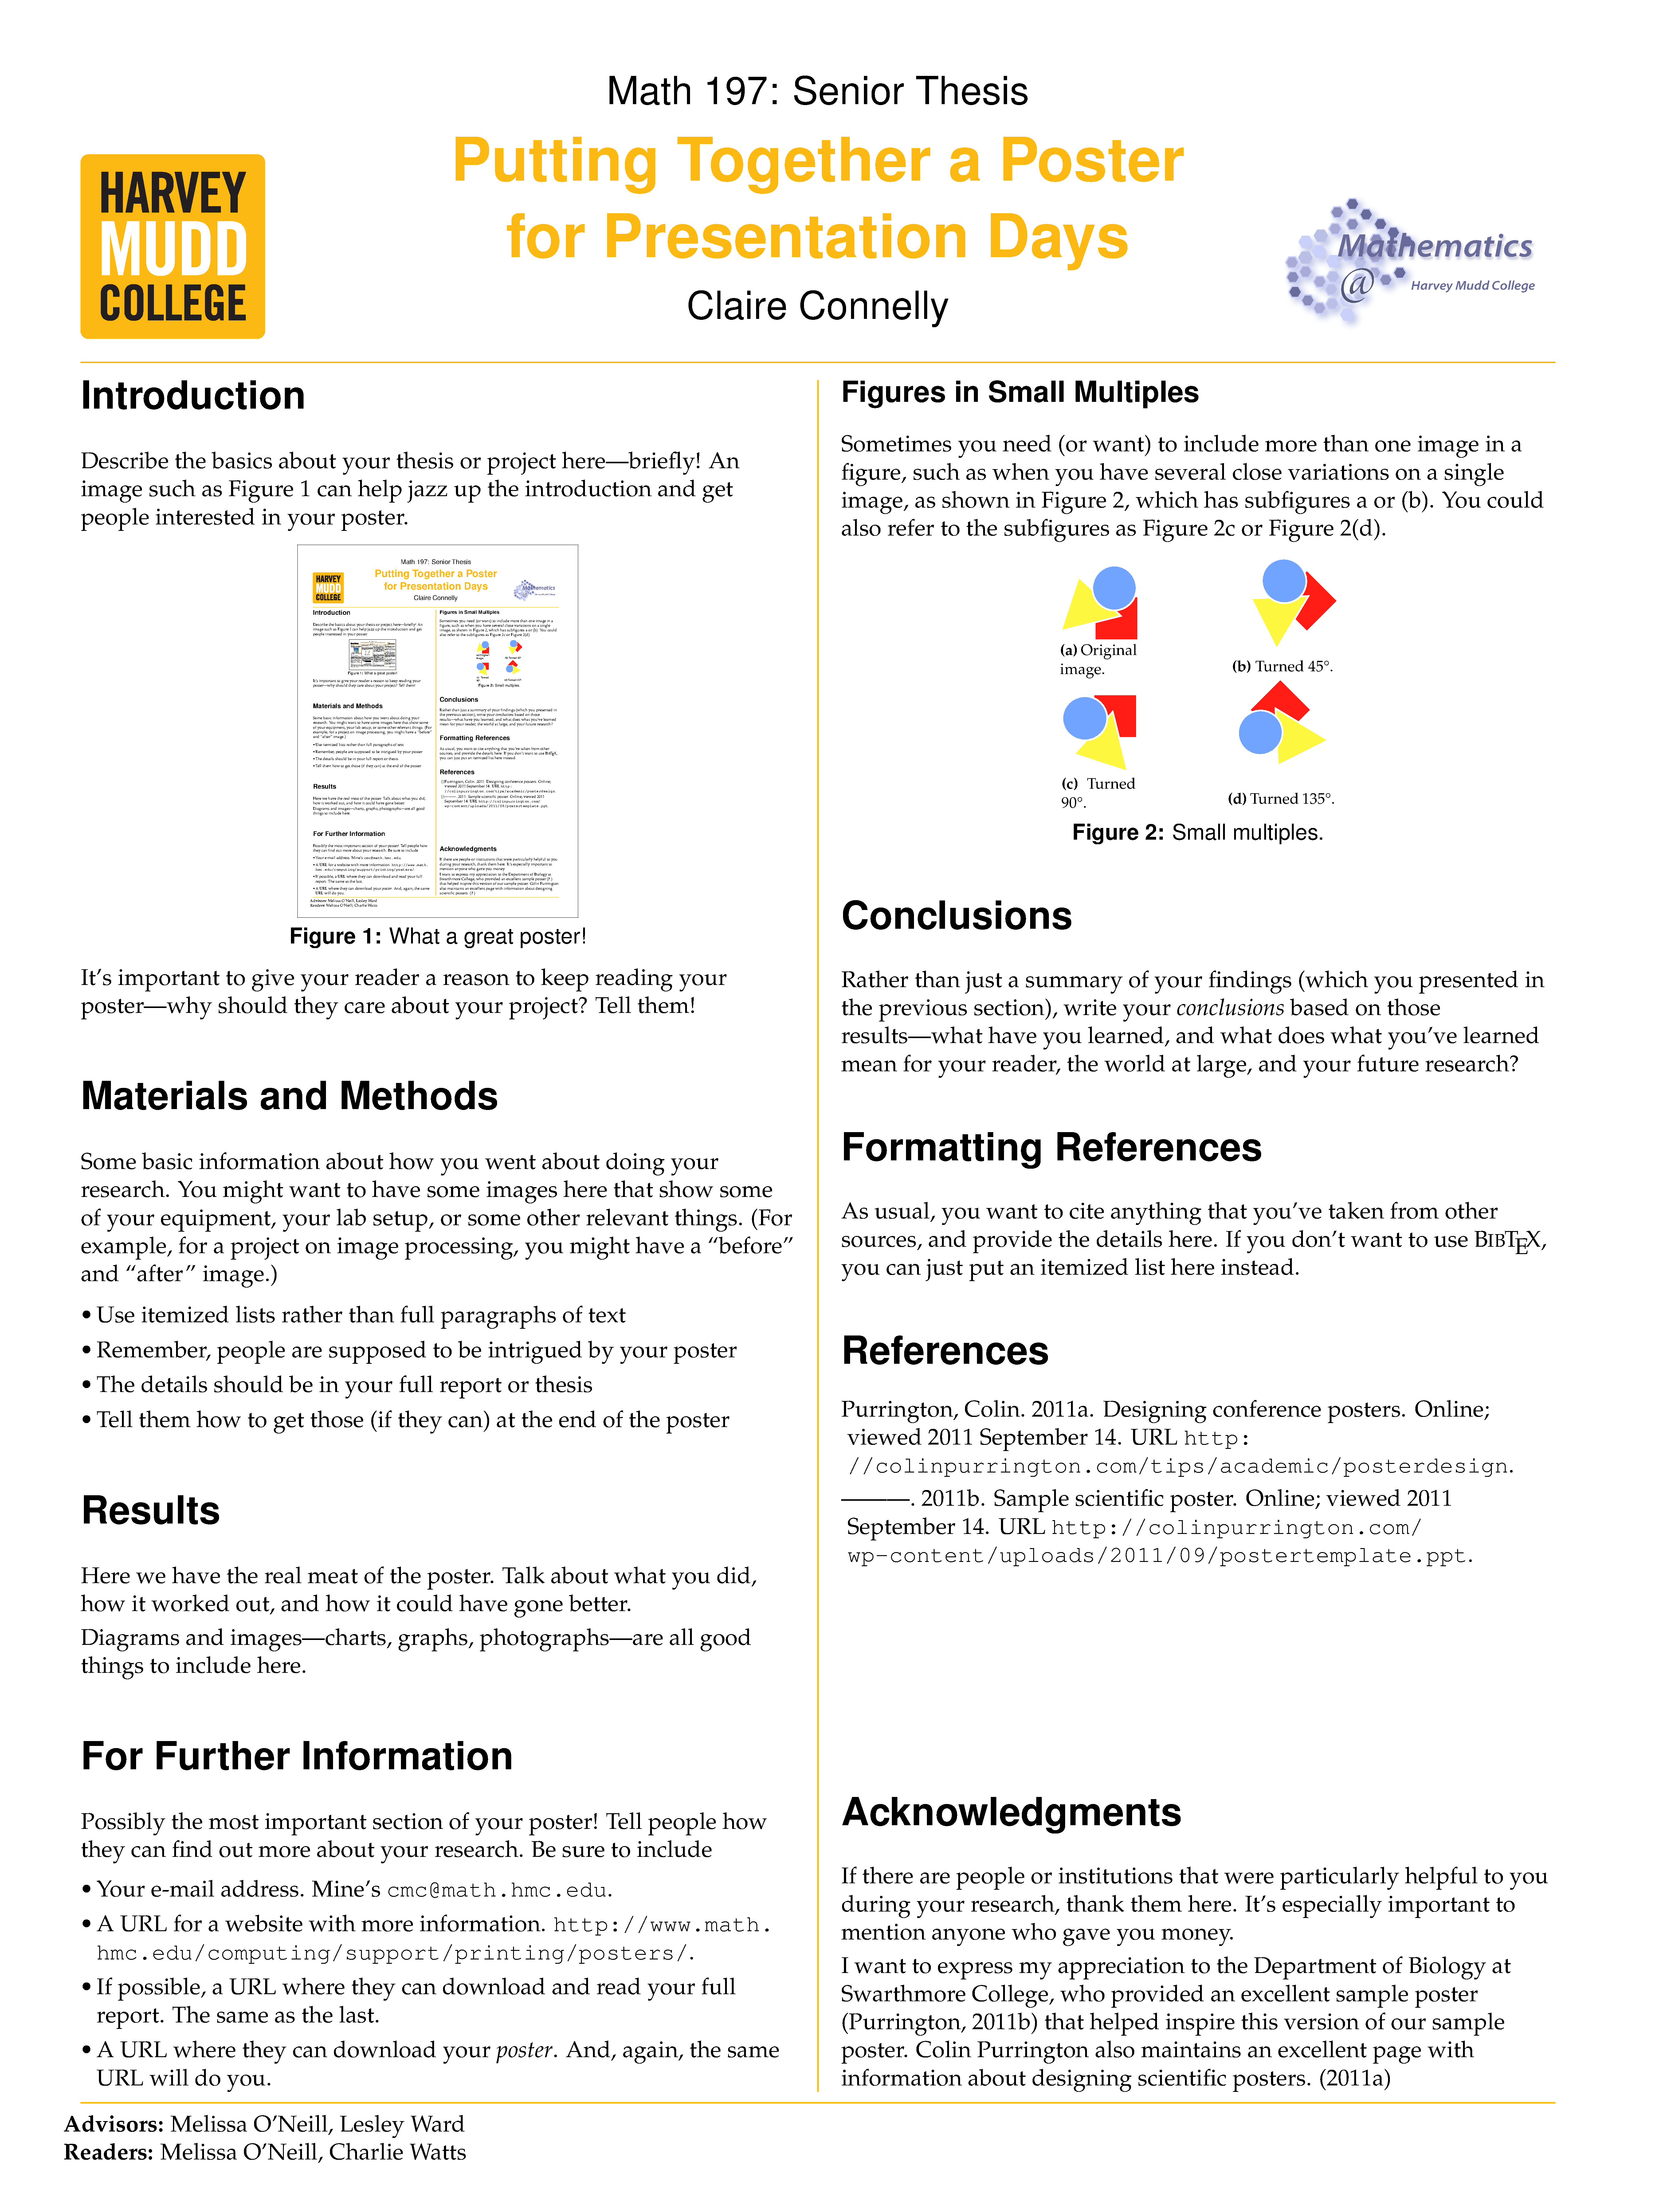
\includegraphics[width=6in]{sampleposter}}
\caption{What a great poster!}%
\label{fig:our-poster}
\end{center}
\end{figure}

It's important to give your reader a reason to keep reading your
poster---why should they care about your project?  Tell them!


\section{Materials and Methods}%

Some basic information about how you went about doing your
research.  You might want to have some images here that show some of
your equipment, your lab setup, or some other relevant things.  (For
example, for a project on image processing, you might have a
``before'' and ``after'' image.)

\begin{itemize}
\item Use itemized lists rather than full paragraphs of text
\item Remember, people are supposed to be intrigued by your poster
\item The details should be in your full report or thesis
\item Tell them how to get those (if they can) at the end of the poster
\end{itemize}


\section{Results}%

Here we have the real meat of the poster.  Talk about what you did,
how it worked out, and how it could have gone better.

Diagrams and images---charts, graphs, photographs---are all good
things to include here.


\section{For Further Information}

Possibly the most important section of your poster!  Tell people
how they can find out more about your research.  Be sure to
include
\begin{itemize}
\item Your e-mail address.  Mine's \url{cmc@math.hmc.edu}.
\item A URL for a website with more information.  \url{http://www.math.hmc.edu/computing/support/printing/posters/}.
\item If possible, a URL where they can download and read your full
  report.  The same as the last.
\item A URL where they can download your \emph{poster}.
\end{itemize}


\vfill
%\columnbreak


\subsection{Figures in Small Multiples}

Sometimes you need (or want) to include more than one image in a
figure, such as when you have several close variations on a single
image, as shown in Figure~\ref{fig:small-multiples}, which has
subfigures \subref*{fig:small-mults-orig} or
\subref{fig:small-mults-45}.  You could also refer to the subfigures
as Figure~\ref{fig:small-mults-90} or
Figure~\ref{fig:small-multiples}\subref{fig:small-mults-135}.

\begin{figure}
  \centering
        \subfloat[][Original image.]{\scalebox{.75}{
\includegraphics{shapes}}%
                \label{fig:small-mults-orig}%
        }\qquad\qquad
        \subfloat[][Turned 45\textdegree.]{
\includegraphics[scale=.75,origin=c,angle=45]{shapes}%
                \label{fig:small-mults-45}%
        }\\
        \subfloat[][Turned 90\textdegree.]{\scalebox{.75}{
\includegraphics[origin=c,angle=90]{shapes}}%
                \label{fig:small-mults-90}%
        }\qquad\qquad
        \subfloat[][Turned 135\textdegree.]{\scalebox{.75}{
\includegraphics[origin=c,angle=135]{shapes}}%
                \label{fig:small-mults-135}%
        }
  \caption[Small multiples]{Small multiples.}%
  \label{fig:small-multiples}
\end{figure}


\section{Conclusions}

Rather than just a summary of your findings (which you presented in
the previous section), write your \emph{conclusions} based on those
results---what have you learned, and what does what you've learned
mean for your reader, the world at large, and your future research?

\section{Formatting References}

As usual, you want to cite anything that you've taken from other
sources, and provide the details here.  If you don't want to use
\bibtex, you can just put an itemized list here instead.

%% References.
%% Note that BibTeX will add its own section-level header, ``References''.

\bibliographystyle{hmcmath}
\bibliography{sampleposter}
\vfill

\section{Acknowledgments}

If there are people or institutions that were particularly helpful
to you during your research, thank them here.  It's especially
important to mention anyone who gave you money.

I want to express my appreciation to the Department of Biology at
Swarthmore College, who provided an excellent sample poster
\citep{swarthmore-poster} that helped inspire this version of our
sample poster.  Colin Purrington also maintains an excellent page
with information about designing scientific
posters. \citeyearpar{purrington-sciposters}

\vfill
\end{poster}

\end{document}

 
